\documentclass[a4paper]{article}
\usepackage[utf8]{inputenc}
\usepackage[russian,english]{babel}
\usepackage[T2A]{fontenc}
\usepackage[left=10mm, top=20mm, right=18mm, bottom=15mm, footskip=10mm]{geometry}
\usepackage{indentfirst}
\usepackage{amsmath,amssymb}
\usepackage[italicdiff]{physics}
\usepackage{graphicx}
\usepackage{multirow}
\usepackage{svg}
\graphicspath{{images/}}
\DeclareGraphicsExtensions{.pdf,.png,.jpg}
\usepackage{wrapfig}
\usepackage{caption}
\captionsetup[figure]{name=Рисунок}
\captionsetup[table]{name=Таблица}
\title{\underline{Петля гистерезиса (динамический метод)}}
\author{Каспаров Николай, Б01-304}

\begin{document}

\maketitle
\begin{center}
\Large{\textbf{ }}
\end{center}

\subparagraph{Цель работы:}

    Изучение петель гистерезиса раличных ферромагнитных
    материалов в переменных токах

\subparagraph{В работе используются:}

    Автотрансформатор, понижающий
    трансформатор, интегрирующая цепочка, амперметр, вольтметр,
    электронный осциллограф, делитель напряжения, тороидальные образцы
    с двумя обмотками (с сердечниками из феррита, пермаллоя и кремнистого
    железа).

\section{Ход работы}

\subsection{Калибровка канала X ЭО}

Закоротим $N_0$, через резистор $R_0$ потечек синусодиальный ток, эффективную величину которого
можно измерить амперметром. Измерив $2x$ - длину горизонтальной прямой на экране, 
можно рассчитать $K_x$ - чувствительность канала X:

\begin{equation}
    K_x = \frac{2R_0 \sqrt{2}I_\text{эф}}{2x} \approx (140 \pm 20) \ \frac{\text{мB}}{\text{дел}}
\end{equation}

\subsection{Калибровка канала Y ЭО}

Аналогично можно откалибровать канал Y:

\begin{equation}
    K_y = \frac{2 \sqrt{2}U_\text{эф}}{2x} \approx (70 \pm 5) \ \frac{\text{мB}}{\text{дел}}
\end{equation}

\subsection{Измерение параметров интегрирующей ячейки}

Постоянная $RC$ нам известна, но её также можно определить и экспериментально.
Как известно из РТ-лаб:
\begin{equation}
    \tau = RC = \frac{U_\text{вх}}{wU_\text{вых}} = (0.43 \pm 0.05) \ c
\end{equation}

Что совпадает с известным значением: $RC = 0.4 \ c$

\newpage

\subsection{Измерения над пермаллоем}
$N_0 = 15 \ \text{витков}$

$N_\text{и} = 300 \ \text{витков}$

$S = 0.66 \ \text{см}^2$

$2 \pi R = 14.1 \text{см}$

\begin{figure}[h!]
    \centering
    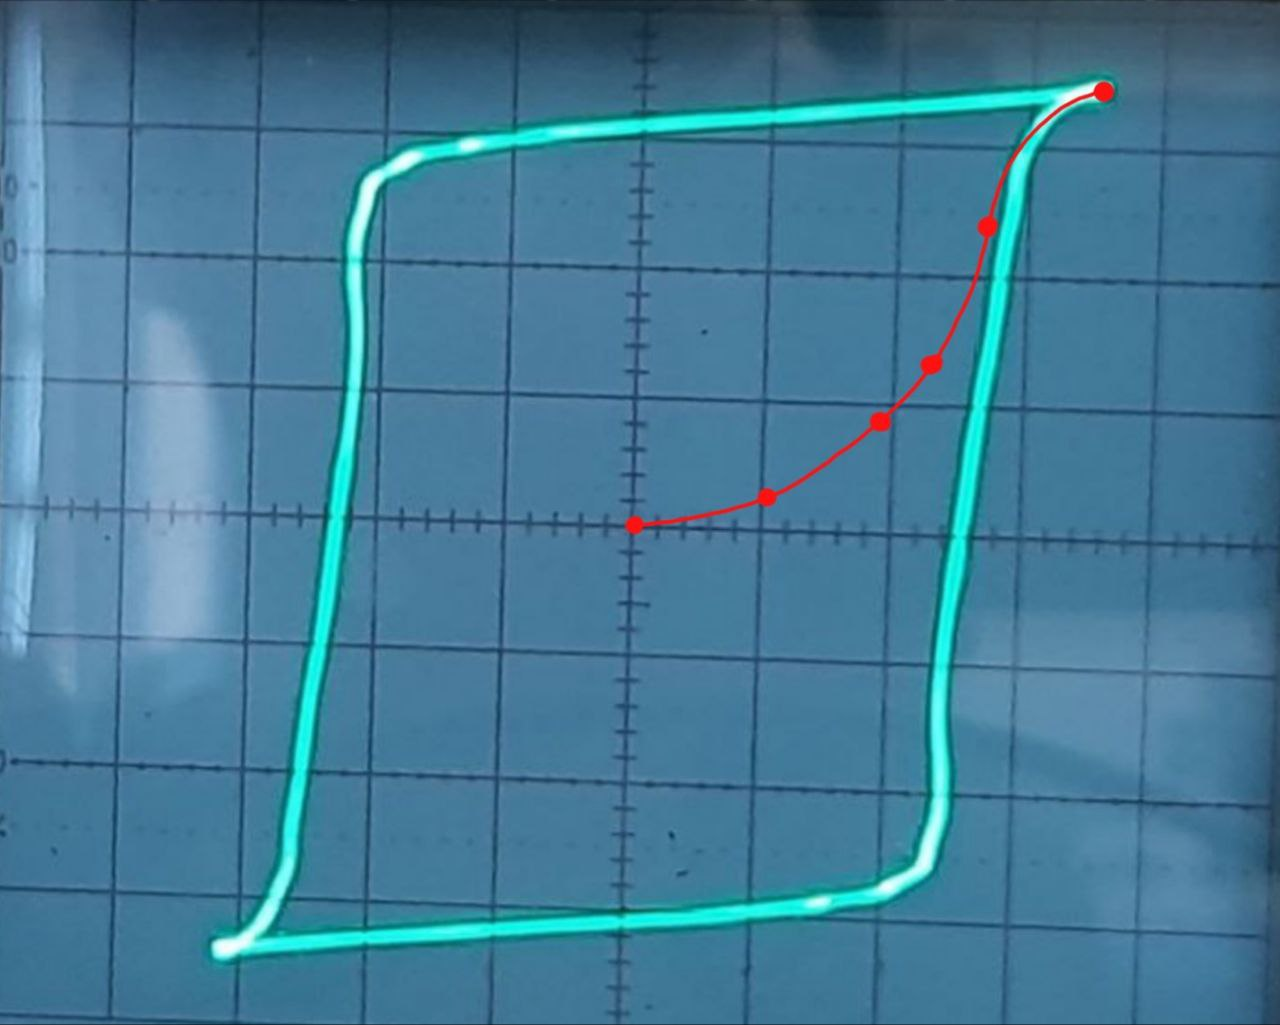
\includegraphics[width=0.5\pdfpagewidth]{12.jpg}
    \caption{Предельная петля гистерезиса для пермаллоя}
\end{figure}

\begin{equation*}
    H = \frac{N_0 K_x}{2\pi RR_0} = (15 \pm 3) \frac{A}{\text{м}} \qquad 
\end{equation*}
\begin{equation*}
    B = \frac{R_\text{и} C_\text{и} K_y}{S N_\text{и}} = (0.70 \pm 0.05) \ \text{Тл}
\end{equation*}

\begin{equation*}
    H_c = (30 \pm 6) \ \frac{A}{\text{м}}
\end{equation*}
\begin{equation*}
    B_s = (1.4 \pm 0.1) \ \text{Тл}
\end{equation*}

\newpage

\subsection{Измерения над ферритом}
$N_0 = 45 \ \text{витков}$

$N_\text{и} = 400 \ \text{витков}$

$S = 3.0 \ \text{см}^2$

$2 \pi R = 25 \text{см}$

\begin{figure}[h!]
    \centering
    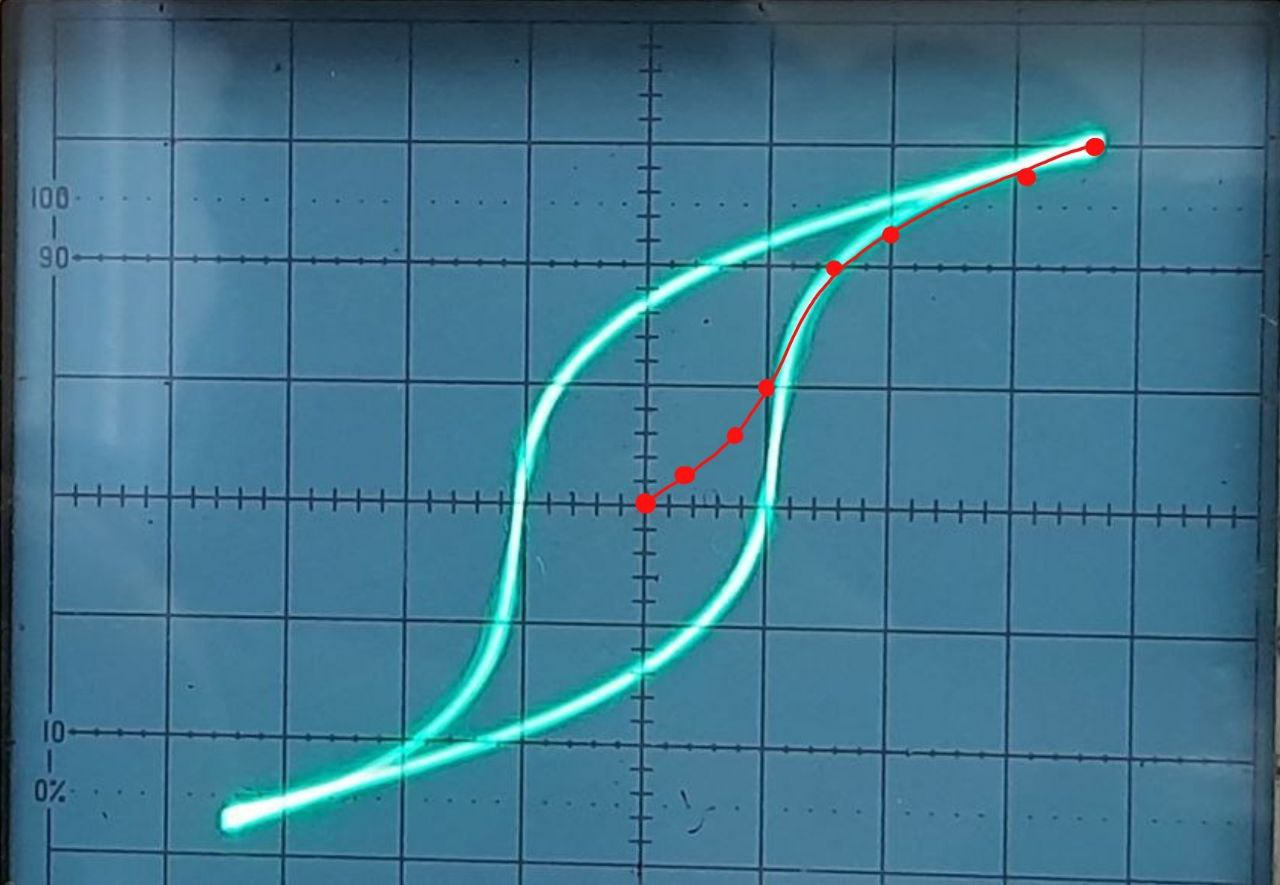
\includegraphics[width=0.5\pdfpagewidth]{11.jpg}
    \caption{Предельная петля гистерезиса для феррита}
\end{figure}

\begin{equation*}
    H = \frac{N_0 K_x}{2\pi RR_0} = (14 \pm 2) \frac{A}{\text{м}} \qquad 
\end{equation*}
\begin{equation*}
    B = \frac{R_\text{и} C_\text{и} K_y}{S N_\text{и}} = (0.19 \pm 0.02) \ \text{Тл}
\end{equation*}

\begin{equation*}
    H_c = (14 \pm 2) \ \frac{A}{\text{м}}
\end{equation*}
\begin{equation*}
    B_s = (0.6 \pm 0.1) \ \text{Тл}
\end{equation*}

\newpage

\subsection{Измерения над кремнистого железа}
$N_0 = 25 \ \text{витков}$

$N_\text{и} = 250 \ \text{витков}$

$S = 2.0 \ \text{см}^2$

$2 \pi R = 11 \text{см}$

\begin{figure}[h!]
    \centering
    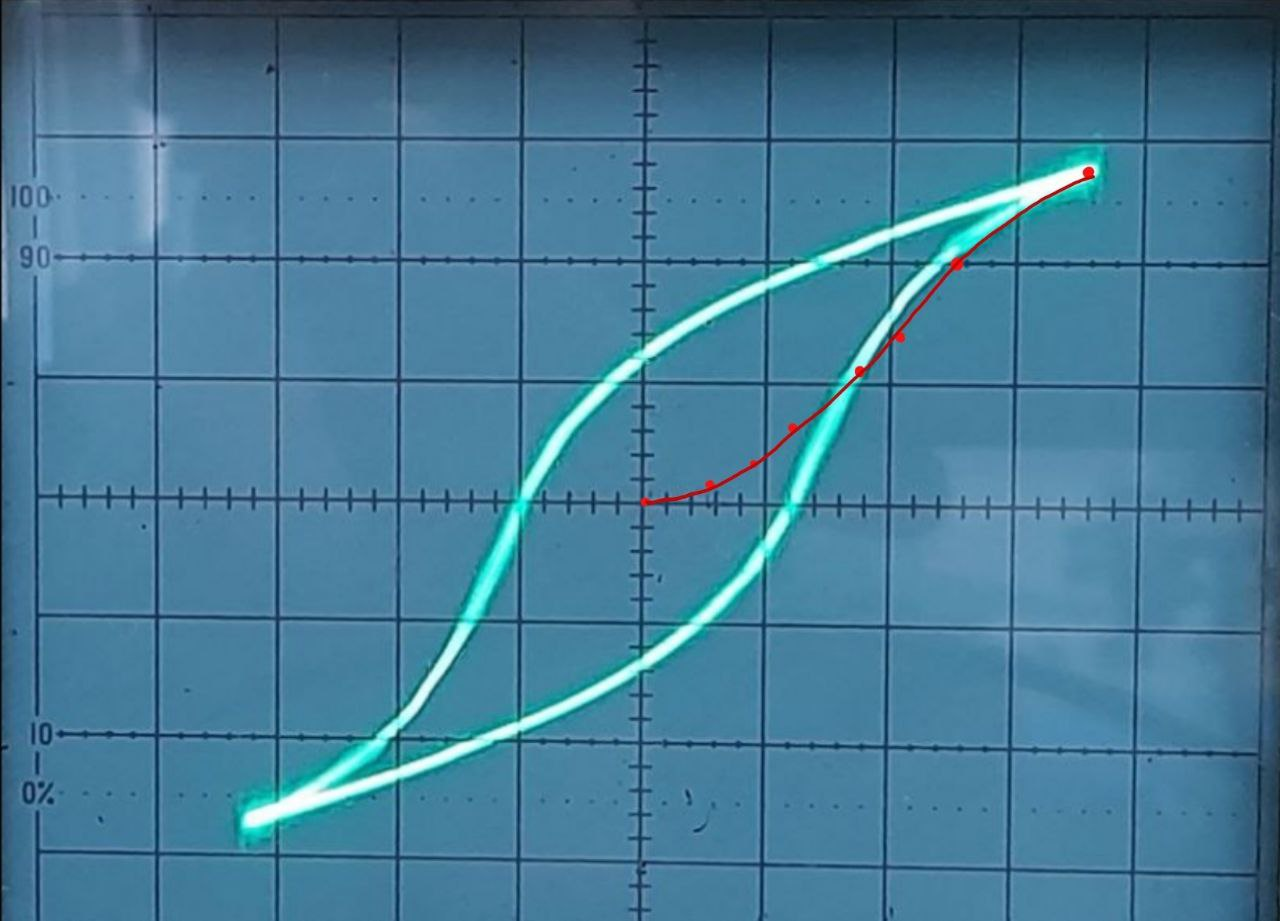
\includegraphics[width=0.5\pdfpagewidth]{13.jpg}
    \caption{Предельная петля гистерезиса для кремнистого железа}
\end{figure}

\begin{equation*}
    H = \frac{N_0 K_x}{2\pi RR_0} = (34 \pm 6) \frac{A}{\text{м}} \qquad 
\end{equation*}
\begin{equation*}
    B = \frac{R_\text{и} C_\text{и} K_y}{S N_\text{и}} = (0.4 \pm 0.1) \ \text{Тл}
\end{equation*}

\begin{equation*}
    H_c = (25 \pm 4) \ \frac{A}{\text{м}}
\end{equation*}
\begin{equation*}
    B_s = (1.2 \pm 0.2) \ \text{Тл}
\end{equation*}

\section{Вывод}

В рамках данной лабораторной работы были изучены петли гистерезиса для трех разных образ-
цов, и для каждого из них были получены характерные величины, которые по порядку величины
совпали с табличными значениями. Также была оценена применимость используемого метода в усло-
виях нашего эксперимента. В результате было подтверждено, что условия применимости соблюдают-
ся, а сам метод является эффективным для определения характерных параметров ферромагнитных
материалов.

\end{document}

